\documentclass[conference]{IEEEtran}
\usepackage{cite}
\usepackage{amsmath,amssymb,amsfonts}
\usepackage{algorithmic}
\usepackage{graphicx}
\usepackage{textcomp}
\usepackage{tikz}


\begin{document}

\title{Reading Assignment XYZ
}

\author{\IEEEauthorblockN{Given Name Surname}
\IEEEauthorblockA{\textit{Dept. of Mathematics and Computer Science} \\
\textit{Karlstad University}\\
Karlstad, Sweden \\
}

}

\maketitle

\begin{abstract}
This document contains some suggestions for a reading assignment report in the course Systems Modeling and Simulation. In your abstract you should write a short description of the high-level objectives in the papers you read, what insights you got, and briefly address any specific aspects given in the assignment specification.

\end{abstract}


\section{Introduction}
In the introduction you can provide a short description of the general area that the papers were about, why it is relevant area, and provide some broader context around it. Some might already have been mentioned in the abstract, but it OK to have some overlap between abstract and introduction. Minimum length of this reading assignment report is one full page, maximum length is two full pages.


\section{Paper review approach}
Here you briefly describe the process you applied to complete the assignment. For example, you may first glance both papers at an overview level, then make a detailed read of each paper while taking notes, and then use then notes to write the text for the assignment. Another alternative may be to make a detailed reading of each paper, then reread the same paper while simultaneously filling in this template. Or, you may do it in any of many other possible ways, so in this section  you describe how YOU did it. Also, you should report the approximate amount of time you spent on this assignment.


\section{Summary of Paper 1}
Here you provide a summary of \cite{b1} (You need to update the reference list).

What is the problem addressed, what are the methods applied, what were the main conclusions arrived at, etc...
Should be kept factual with no personal reflections or opinions expressed.

\section{Reflections on Paper 1}
Here you elaborate on what insights you got, and address  any specific aspects given in the assignment specification.



\section{Summary of Paper 2}
Same as above, but for \cite{b2}.

\section{Reflections on Paper 2}
Same as above, but for \cite{b2}.

\section{Summary of assignment and Conclusions}
Write a few sentences to summarize the assignment.





\begin{thebibliography}{00}
% here are some examples of references. If you know the bibtex workflow it might be better to use that instead of lines with bib items. It is not necessary to
% abbreviate the journal names as done in some examples below.
% Note that in your report any line included in the reference list must be referred to in the text of the report.
\bibitem{b1} G. Eason, B. Noble, and I. N. Sneddon, ``On certain integrals of Lipschitz-Hankel type involving products of Bessel functions,'' Phil. Trans. Roy. Soc. London, vol. A247, pp. 529--551, April 1955.
\bibitem{b2} Y. Yorozu, M. Hirano, K. Oka, and Y. Tagawa, ``Electron spectroscopy studies on magneto-optical media and plastic substrate interface,'' IEEE Transl. J. Magn. Japan, vol. 2, pp. 740--741, August 1987 [Digests 9th Annual Conf. Magnetics Japan, p. 301, 1982].
\end{thebibliography}

%%The stuff below should be removed, make sure to keep the final \end{document} line though!
\section*{Appendix}
In most cases there is no need to include equations, figures or tables in an assignment report such as this one. In case you nevertheless find it valuable to include some table or figure these work as examples of how it can be done.

Equations can be included, as for example:
\begin{equation}
a+b=\gamma\label{eq1}
\end{equation}

You can refer to equations in the text as Eq. \eqref{eq1}.



% More documentation on tables:
%https://www.overleaf.com/learn/latex/tables
\begin{table}[b]
  \begin{center}
    \caption{Experimental results.}
    \label{tab:table1}
    \begin{tabular}{l|c|c}
      \textbf{Experiment} & \textbf{Config A} & \textbf{Config B}\\
      \hline
      1 & 11.1 & 12.3\\
      2 & 10.1 & 13.4\\
      3 & 23.3 & 26.7\\
      4 & 25.3 & 24.1\\
    \end{tabular}
  \end{center}
\end{table}



\begin{figure}[tb]

%Typically you would import some file to show, using a line like the commented below :
%\centerline{\includegraphics[width=0.98\columnwidth]{BoxplotCompletionTime.pdf}}


%However, since I don't want to shuffle around files for this, you instead get an optical illusion as an example figure....

\resizebox{0.78\columnwidth}{!}{%
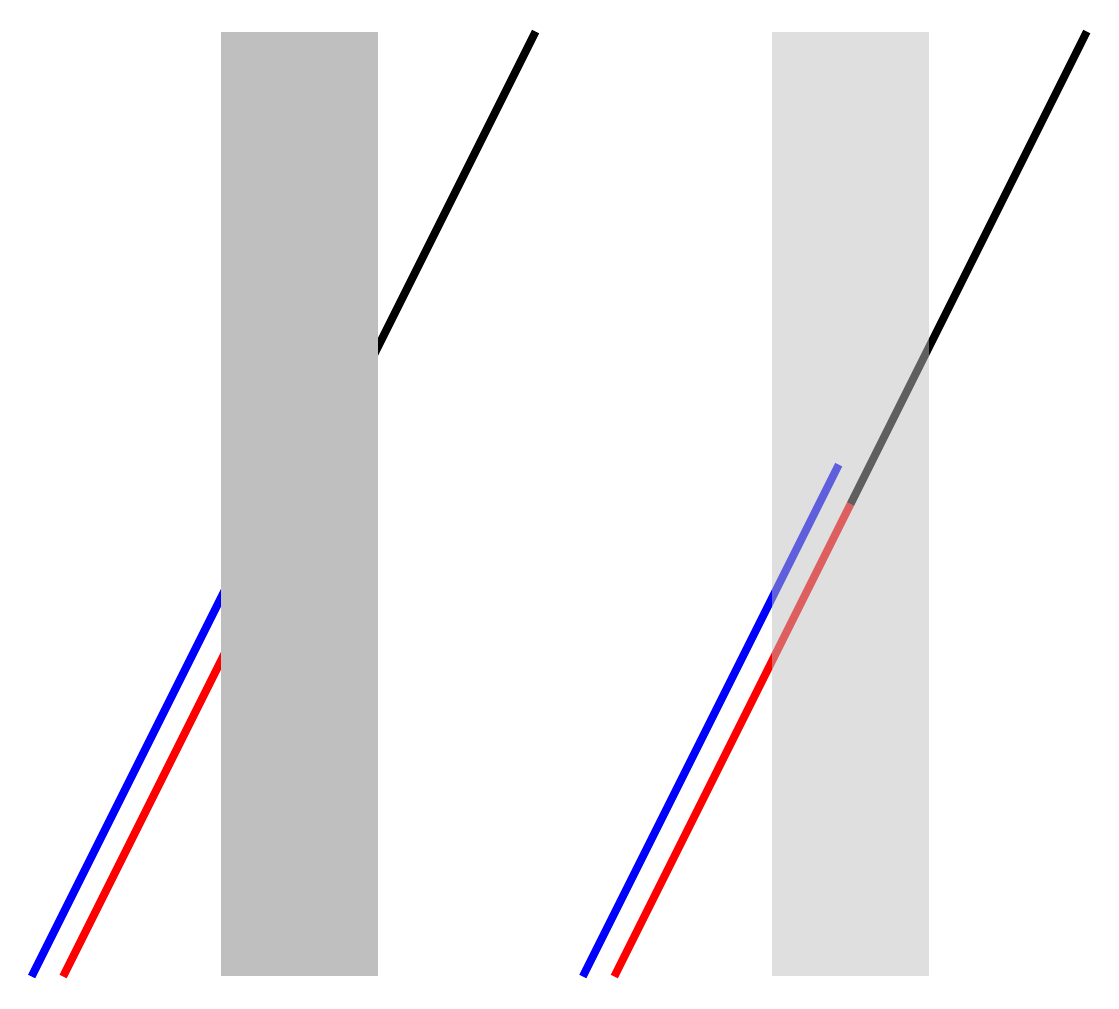
\begin{tikzpicture}[line width=1mm]

% Left side illustration

\draw [red] (0,0) -- ++ (3,6);
\draw (3,6) -- ++ (3,6);
\draw [blue] (-0.4,0) -- ++ (3.25,6.5);

% rectangle
\fill[lightgray] (2,0) rectangle ++(2,12);

% Right side illustration

\begin{scope}[xshift=7cm]
\draw [red] (0,0) -- ++ (3,6);
\draw (3,6) -- ++ (3,6);
\draw [blue] (-0.4,0) -- ++ (3.25,6.5);

% rectangle
\fill[lightgray,opacity=0.5] (2,0) rectangle ++(2,12);
\end{scope}

\end{tikzpicture}
}


\caption{Example figure showing the Poggendorff illusion}
\label{figlabel}
\end{figure}



Figure captions should be
below the figures; table heads should appear above the tables.
Use
``Figure~\ref{figlabel}'' to reference a figure, and always use a capital F.


In case you want to include a bullet lists, this is how you do it:
\begin{itemize}
\item First insight ...
\item Second insight ...
\end{itemize}




\end{document}
